\documentclass[12pt]{article}
\usepackage[top=1in,left=1in, right = 1in, footskip=1in]{geometry}

\title{Using sequence data to inform antigenic map}
\usepackage{graphics}
\usepackage{adjustbox}

\newcommand{\eref}[1]{(\ref{eq:#1})}
\newcommand{\fref}[1]{Fig.~\ref{fig:#1}}
\newcommand{\Fref}[1]{Fig.~\ref{fig:#1}}
\newcommand{\sref}[1]{Sec.~\ref{#1}}
\newcommand{\frange}[2]{Fig.~\ref{fig:#1}--\ref{fig:#2}}
\newcommand{\tref}[1]{Table~\ref{tab:#1}}
\newcommand{\tlab}[1]{\label{tab:#1}}

\usepackage{amsthm}
\usepackage{amsmath}
\usepackage{amssymb}
\usepackage{amsfonts}

\usepackage{hyperref}
\usepackage{natbib}
\usepackage{hyperref}
\bibliographystyle{chicago}
\date{\today}

\usepackage{xspace}
\newcommand*{\ie}{i.e.\@\xspace}

\usepackage{color}

\newcommand{\Rx}[1]{\ensuremath{{\mathcal R}_{#1}}} 
\newcommand{\Ro}{\Rx{0}}
\newcommand{\RR}{\ensuremath{{\mathcal R}}}
\newcommand{\tsub}[2]{#1_{{\textrm{\tiny #2}}}}
\newcommand{\tsup}[2]{#1^{{\textrm{\tiny #2}}}}


\newcommand{\comment}[3]{\textcolor{#1}{\textbf{[#2: }\textsl{#3}\textbf{]}}}
\newcommand{\jd}[1]{\comment{cyan}{JD}{#1}}
\newcommand{\swp}[1]{\comment{magenta}{SWP}{#1}}
\newcommand{\hotcomment}[1]{\comment{red}{HOT}{#1}}

\begin{document}
\maketitle

\section*{Data}

\begin{itemize}
	\item Titer data from \cite{bedford2014integrating}
	\item HA amino acid sequence data from GISAID and IRD (wasn't able to get one of the sequences so I removed it from titer data as well)
\end{itemize}

\section*{Antigenic map based on sequences}

\begin{itemize}
	\item Align sequences using the DECIPHER package \citep{wright2016using}. This package performs what they call ``profile-to-profile'' alignment by constructing a tree and alining with respect to the tree; this process is repeated until convergence and some? subset of the alignments are re-aligned based on sum-of-pairs scores. Repeated until convergence.
	\item Use Hamming distance to compare sequence in 5 regions: Sa, Sb, Ca1, Ca2, and Cb \citep{anderson2018antigenic}. For each region, the Hamming distance is divided by the length of regions and the proportions are averaged across 5 regions. These distances are multiplied by 20 to reflect 20-dimensional immunological shape space described by Smith et al.; this seems kind of arbitrary to me but let's see what happens.
	\item Classical MDS based on these distances
\end{itemize}

First, here are 5 maps based on 5 different regions (\fref{ind}).
We see slightly different patterns across regions.
Overall, there seems to be a circular pattern in each of them?
We see similar (but slightly different geometrically) circular when we use the averaged distance (\fref{avg}).
\cite{anderson2018antigenic} used a lot more sequence data to create the same map; we can see similar circular patterns in their analysis.

\begin{figure}
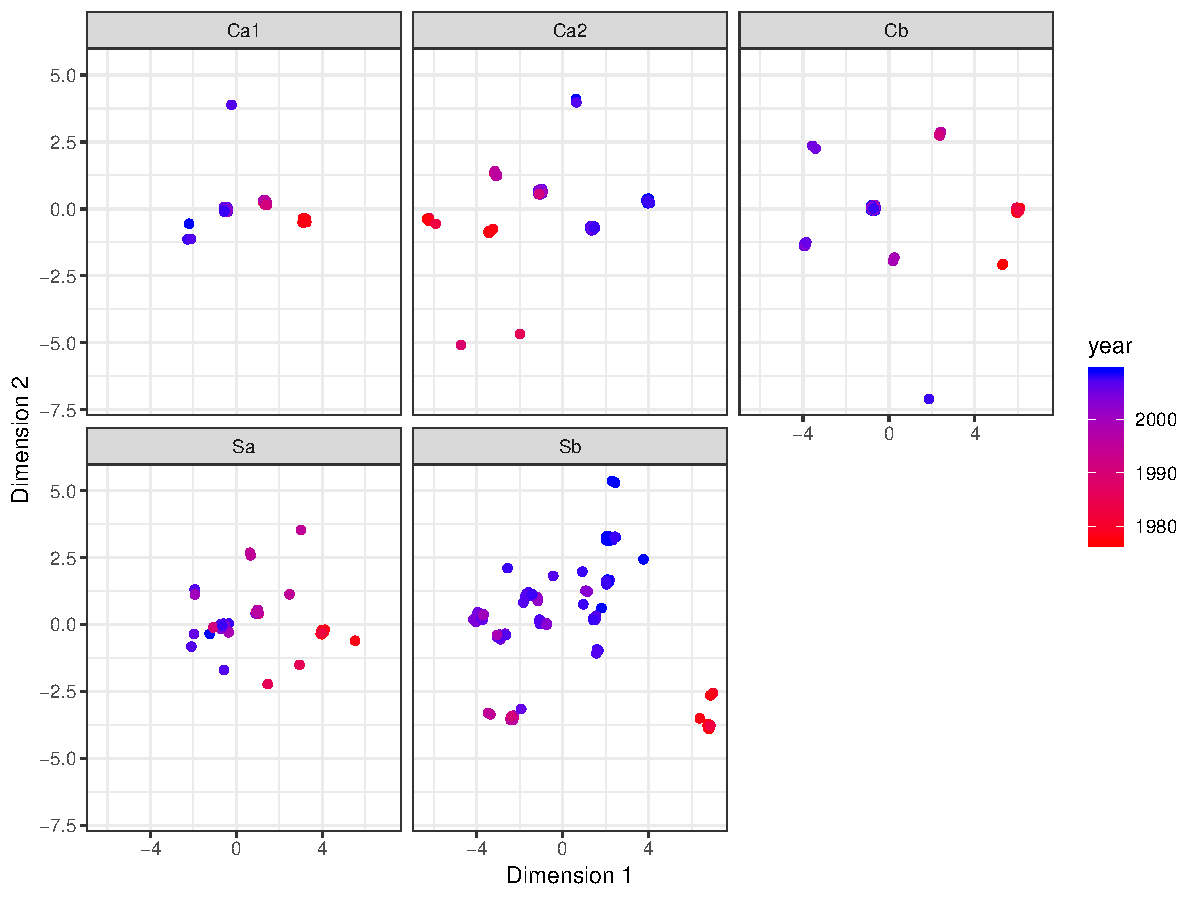
\includegraphics[width=\textwidth]{../figure/individual_map.pdf}
\label{fig:ind}
\caption{Antigenic map based on Hamming distance (measured as proportion of mutations) across 5 regions. Points are jittered to show overlapping points.}
\end{figure}

\begin{figure}
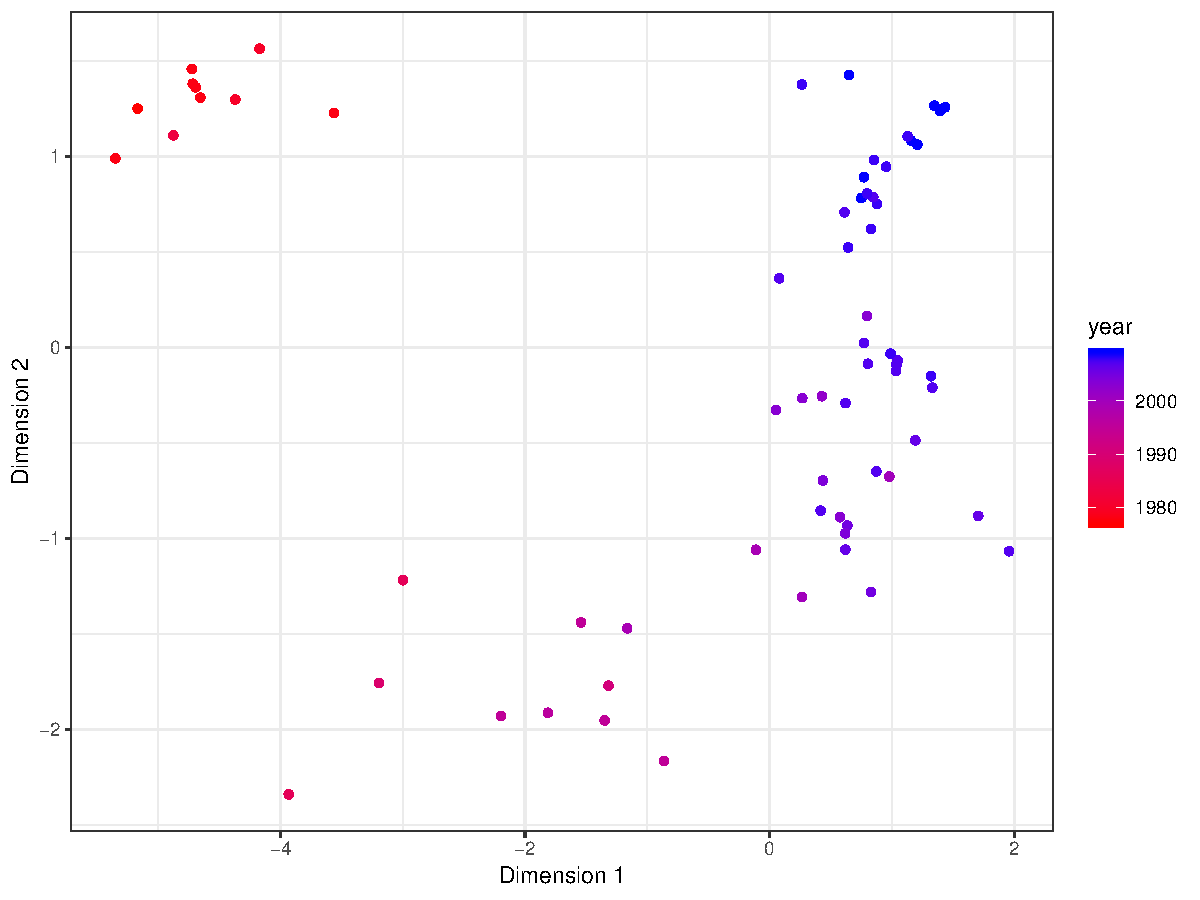
\includegraphics[width=\textwidth]{../figure/average_map.pdf}
\label{fig:avg}
\caption{Antigenic map based on mean Hamming distance (measured as proportion of mutations) across 5 regions}
\end{figure}

We want to be able to use this map to inform our antigenic maps based on HI titers. We're going to call these locations $\mu_i$, where each $\mu_i$ is a 2-dimensional vector (can be generalized into $D$ dimensions).
Then, the location of virus $X_i$ and the location of serum $Y_i$ can be assigned multivariate normal priors:
\begin{equation}
X_i \sim \mathcal{N}(\mu_i, \Sigma_r), Y_i \sim \mathcal{N}(\mu_i, \Sigma_r)
\end{equation}
where $\Sigma_r$ is a diagonal matrix whose entries are $\sigma_r^2$.
I think it's better to think of $\sigma_r^2$ as a penalization term rather than trying to find a posterior for it. 
We might be able to try multiple values of $\sigma_r^2$ and do something analogous to cross validation? Not sure yet.
For now, I assumed that $\sigma_r^2 = 0.5$ such that the Euclidean distance between a homologous virus and serum will be less than 2 (1.96, technically) \textit{a priori} with 95\% probability. This means that homologous pair can have 95\% prior probability of having up to 4 fold difference in HI titers with respect to the maximum titer, in the absence of effect of virus or effect of serum.
This seems like a biologically reasonable range and a decent amount of penalization? We could try other values later.

Finally, we can model log2 HI titer as usual:
\begin{equation}
HH_{i,j} \sim \mathcal{N}\left(\beta_0 - d(X_i, Y_j) + J_i + A_j, \sigma^2\right),
\end{equation}
where 
\begin{equation}
\begin{aligned}
J_i &\sim \mathcal{N}(0, \sigma_J^2)\\
A_j &\sim \mathcal{N}(0, \sigma_A^2)\\
\sigma_J &\sim \mathrm{Gamma}(5, 5)\\
\sigma_A &\sim \mathrm{Gamma}(5, 5)\\
\sigma &\sim \mathrm{Half-Cauchy}(0, 10)\\
\beta_0 &\sim \mathcal{N}(0, 5)\\
\end{aligned}
\end{equation}
We should weaken some of these priors later. For now, I'm trying out priors that are not too weak as a preliminary analysis.

Results are summarized in \fref{compare}.
We can see that there are noticeable shifts in the location of virus strains. A lot of them don't seem to move around too much but the ones in 1980's seem to move around a lot.
Taking HI titres into account seems to preserve the circular patterns (with respect to time) in the map.

\begin{figure}
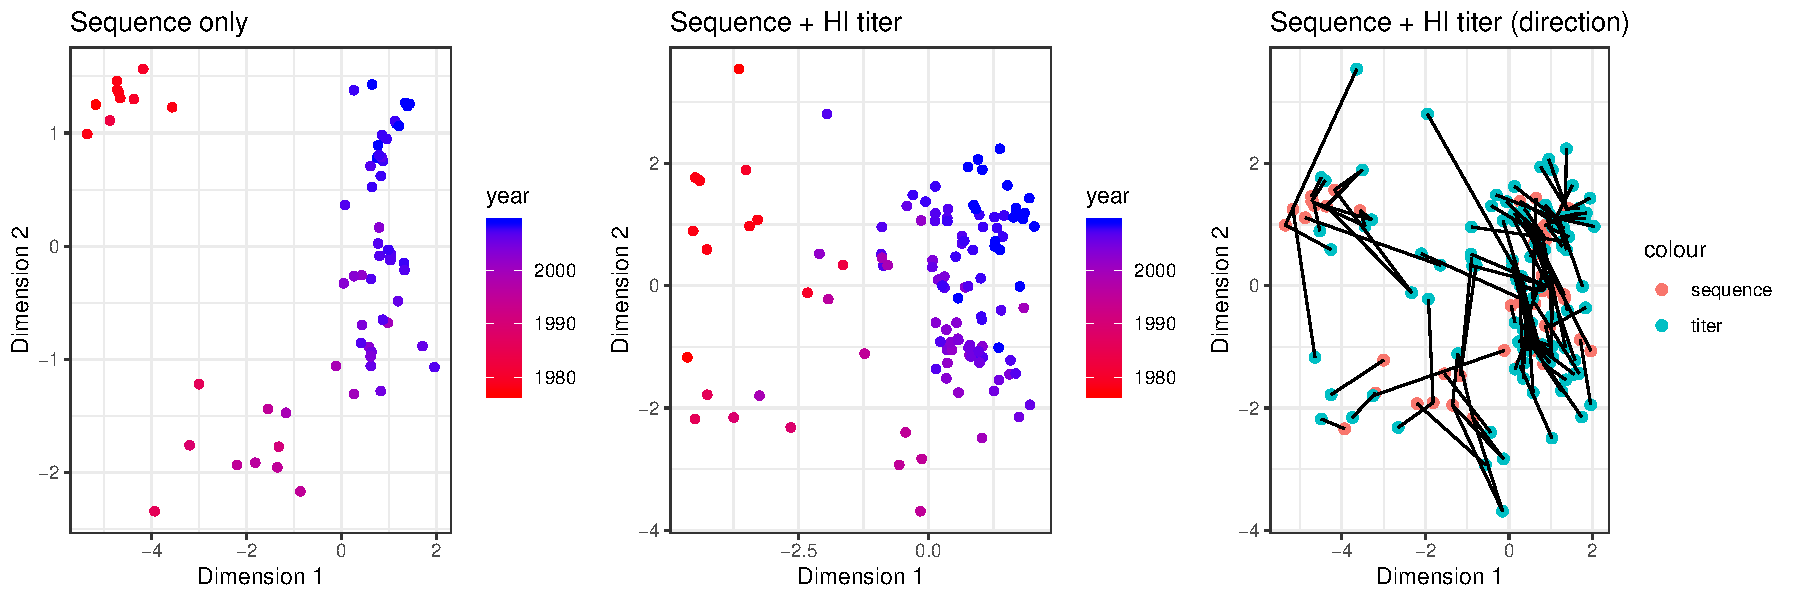
\includegraphics[width=\textwidth]{../figure/h1n1_hamming_informed_map.pdf}
\label{fig:compare}
\caption{Sequence only: antigenic map based on mean Hamming distance (measured as proportion of mutations) across 5 regions. Sequence + HI titer: antigenic map based on HI titer informed by the sequence map; only showing posterior median. Sequence + HI titer (direction): solid lines connect the virus locations based on the sequence (prior mean) with the locations of the same virus based on HI titres (posterior median).}
\end{figure}

See \fref{eff} for effects of virus and antisera.
These patterns are very similar to the patterns that we saw before when we didn't use the sequence data.
Virus effect seems to decrease over time. There's a weird jump in 2005.
Antiserum effect stays constant on average with weird jumps around 2003-2007.

TODO?
\begin{itemize}
	\item Get more sequences even if we don't have their titre data?
	\item Better distance metrics based on homology models? Or is hamming distance ``good enough''?
	\item Try to interpret virus effects and serum effects?
\end{itemize}

\begin{figure}
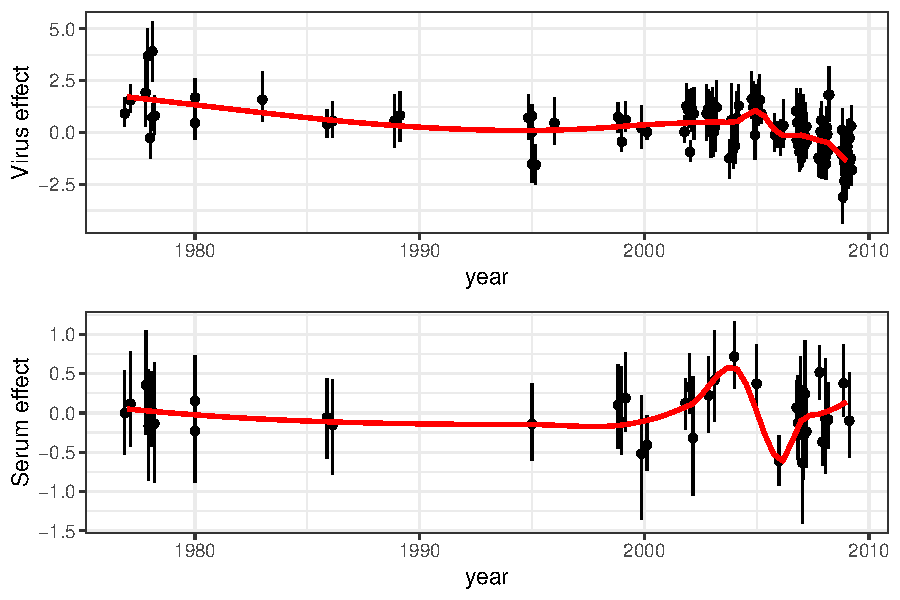
\includegraphics[width=\textwidth]{../figure/h1n1_hamming_informed_effect.pdf}
\label{fig:eff}
\caption{Estimated effects of virus and effects of antisera over time using HI titre data + the sequence data. Showing posterior median and 95\% credible intervals.}
\end{figure}

\pagebreak

\bibliography{bayes}

\end{document}
